\documentclass{article}[12pt,a4paper]

%!TEX root = main.tex

\def\finex{{\unskip\nobreak\hfil
\penalty50\hskip1em\null\nobreak\hfil{\Large $\diamond$}
\parfillskip=0pt\finalhyphendemerits=0\endgraf}}

\newenvironment{lmref}[1]{%
	\vspace*{0.3cm}
	\noindent {\bf  Lemma #1.}}

\newenvironment{thref}[1]{%
	\vspace*{0.3cm}
	\noindent {\bf  Theorem #1.}}

\newenvironment{corref}[1]{%
	\vspace*{0.3cm}
	\noindent {\bf  Corollary #1.}}


\newcommand{\picalc}{$\pi$-calculus~}
\newcommand{\ms}[1]{\mathsf{#1}}
\newcommand{\ctx}{\mathtt{C}}
\newcommand{\co}[1]{\overline{#1}}
\newcommand{\proj}[1]{\mathtt{proj}(#1)}
\newcommand{\projs}[1]{\mathtt{proj_n}(#1)}
\newcommand{\lts}[1]{\xrightarrow{#1}}
\newcommand{\comm}[1]{\textcolor{blue}{#1}}
\newcommand{\red}[1]{\textcolor{red}{#1}}
\newcommand{\key}{\mathtt{keys}}
\newcommand{\flts}[1]{\overset{#1}\twoheadrightarrow}
\newcommand{\rev}{^{\bullet}}
%\newcommand{\forw}{_{\twoheadrightarrow}}
\newcommand{\eq}{\sim} 
\newcommand{\env}{\theta} 
\newcommand{\ex}{e} 
\newcommand{\proc}[3]{\langle #1,#2,#3\rangle } 
\newcommand{\erl}[1]{\hookrightarrow_{#1}} 
\newcommand{\mem}[2]{[#1\;;#2]}
\newcommand{\bl}[1]{\textcolor{blue}{#1}}
\newcommand{\rd}[1]{\textcolor{red}{#1}}
\newcommand{\mtt}[1]{\mathtt{#1}}
\newcommand{\pid}{\mathtt{pid}}
\newcommand{\procl}[4]{\langle #1,#2,#3,#4\rangle } 
\newcommand{\con}{\equiv}
\newcommand{\conk}{\equiv_k}
\newcommand{\extcon}{\equiv_c}
\newcommand{\de}{\delta}
\newcommand{\G}{\Gamma}
\newcommand{\logg}[1]{\rightharpoonup_{#1}}
\newcommand{\rlogg}[1]{\leftharpoondown_{#1}}
\newcommand{\la}{\lambda}
\newcommand{\col}[1]{\mathtt{col}(#1)}
\newcommand{\rel}{\mathcal{R}}
\newcommand{\conc}{\smile_c}
\newcommand{\nil}{{\bf{0}}}
%\newcommand{\res}{\nu}
\newcommand{\res}[1]{\nu #1\,}
\newcommand{\out}[1]{\langle #1\rangle}
\newcommand{\cont}{\triangleright}
\newcommand{\sub}[2]{\{#1/#2\}}
\newcommand{\op}{op_n}
\newcommand{\pidd}{Pid}
\newcommand{\fmod}{\rightarrowtail}
\newcommand{\enc}[1]{\llparenthesis #1 \rrparenthesis}
\newcommand{\blt}{\bullet}
\newcommand{\str}{C}
\newcommand{\term}[1]{T[#1]}
\newcommand{\en}[1]{\Lbag #1 \Rbag}
\newcommand{\signal}[1]{\{ #1\}}
\newcommand{\systset}{\mathbb{S}}
\newcommand{\confset}{\mathbb{C}}
\newcommand{\set}[1]{\{ #1\}}
\newcommand{\node}[3]{#1,#2\mkern-3mu:\mkern-3mu[\mkern-6mu[#3]\mkern-6.2mu]}


\usepackage{listings}
\usepackage[version=3]{mhchem} % Package for chemical equation typesetting
\usepackage{siunitx} % Provides the \SI{}{} and \si{} command for typesetting SI
\usepackage{algorithm}
\usepackage{algpseudocode}
% units
\usepackage{fancyvrb}
\usepackage{hyperref}
\usepackage{breakurl}             % Not needed if you use pdflatex only.
\usepackage{underscore}           % Only needed if you use pdflatex.
\usepackage{microtype}%if unwanted, comment out or use option "draft"
\usepackage{amssymb}
\setcounter{tocdepth}{3}
\usepackage{graphicx}
\usepackage{listings}
\usepackage{color}
\usepackage{rotating}
\usepackage{todonotes}
\usepackage{mathpartir}
\usepackage{url}
\usepackage{tikz}
\usepackage{amsmath}
\usepackage{stmaryrd}
\usepackage{amsthm}
\usepackage{float}
\usepackage{hyperref}
\usepackage{thm-restate}
\usetikzlibrary{matrix}

\renewcommand{\labelenumi}{\alph{enumi}.} % Make numbering in the enumerate environment by letter rather than number (e.g. section 6)

\theoremstyle{definition}
\newtheorem{example}{Example}[section]
\newtheorem{theorem}{Theorem}

\newtheorem{case}{Case}

\newtheorem{definition}{Definition}
\newtheorem{lemma}{Lemma}
\newcommand{\paral}{\;|\;}
\newcommand{\cons}{\mbox{:}}

\usetikzlibrary{calc,decorations.pathmorphing,shapes}
\newcounter{sarrow}
\newcommand\blts[1]{%
  \stepcounter{sarrow}%
  \mathrel{\begin{tikzpicture}[baseline= {( $ (current bounding box.south) + (0,-0.5ex) $ )}]
      \node[inner sep=.5ex] (\thesarrow) {$\scriptstyle #1$};
      \path[draw,<-,decorate,
      decoration={zigzag,amplitude=1.2pt,segment length=1.5mm,pre=lineto,pre length=6pt}]
      (\thesarrow.south east) -- (\thesarrow.south west);
    \end{tikzpicture}}%
}
\algnewcommand\algorithmicforeach{\textbf{for each}}
\algdef{S}[FOR]{ForEach}[1]{\algorithmicforeach\ #1\ \algorithmicdo}


\begin{document}

\section{Consistency}

\begin{figure}
  \centering
  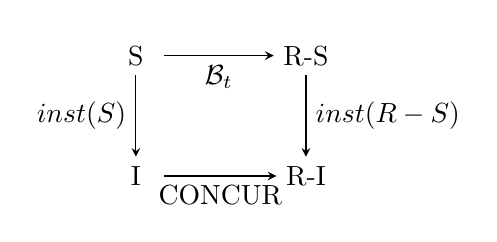
\begin{tikzpicture}
    \centering \matrix (m) [matrix of math nodes,row sep=3em,column
    sep=4em,minimum width=2em] {
      \text{S} & \text{R-S} \\
      \text{I} & \text{R-I} \\}; \path[-stealth] (m-1-1) edge node [left]
    {$inst(S)$} (m-2-1) edge node [below] {$\mathcal{B}_t$} (m-1-2)
    (m-2-1.east|-m-2-2) edge node [below] {$\text{CONCUR}$} node [] {} (m-2-2)
    (m-1-2) edge node [right] {$inst(R-S)$} (m-2-2);
  \end{tikzpicture}
  \caption{ Relation occurring between schemas and instances. }
  \label{fig:square}
\end{figure}

In Fig.~\ref{fig:square} we can observe the relation occurring between schemas
and instances. On the top-left corner we have non-reversible schemas, on the
top-right we have reversible schemas, while below on the
bottom-right corner we have concrete non-reversible instances - i.e., ground
rules - and on the bottom-left corner we have concrete reversible instances.

Schemas differ from instances as they admit the presence of meta-variables that
can range over ground terms. Intuitively, to get from one of the top corners to
the respective concrete one we need to instantiate each meta-variable with
the appropriate ground instance. The correctness of the rule is then ensured by
the set of equations each rule is equipped with, if the concrete instances of
the meta-variables satisfy the equational condition then the instance of the
rule is to be considered correct.\\

Now, let us discuss the top-arrow, that is transforming a non-reversible schema in reversible
schema. A non-reversible schema has the following shape:
\[t \rightarrow t'~\ms{if}~\overline{eq}_n\]
where $t$ and $t'$ are inductively defined as
\[
  \begin{array}{l}
    t,t',t_1,\ldots,t_n: \ms{System} ::=\\
    \hspace{1ex}|~E: \ms{Entity}\\
    \hspace{1ex}|~op(t_1,\ldots,t_n): \ms{System}\\
  \end{array}
\]

Now, for a schema to be reversible each entity must be tagged with a key and a
memory has to be produced each time that a transition is performed. In symbols
\[t_r \rightarrow t'_r \paral \mu ~\ms{if}~\overline{eq}_n\]

Where $t_r$ and $t'_r$ are inductively defined as
\[
  \begin{array}{l}
    t_r,t'_r,t_{1r},\ldots,t_{nr}: \ms{RevSystem} ::=\\
    \hspace{1ex}|~E*K: \ms{Entity} \times \ms{Key}\\
    \hspace{1ex}|~op(t_{1r},\ldots,t_{nr}): \ms{RevSystem}\\
  \end{array}
\]
and $\mu$ is defined as $[R;C]$ where $R$ is the configuration that gave rise to
the step, i.e., $t_r$ and $C$ is a context describing the structure of the
resulting one, where entities have been removed while keys are kept.

Let us now define an auxiliary function.
\[
  \begin{array}{l}
  cmp(t,t_r):\ms{Bool} ::=\\
    \hspace{2ex}\ms{match}~t~\ms{with}\\
    \hspace{4ex}| E: \ms{Entity} \rightarrow \ms{match}~t_r~\ms{with}\\
    \hspace{6ex}| E*K: \ms{Entity}\times\ms{Key}~\rightarrow~true\\
    \hspace{6ex}| \_ \rightarrow false\\
    \hspace{4ex}| op(t_1,\ldots,t_n): \ms{System} \rightarrow \ms{match}~t_r~\ms{with}\\
    \hspace{6ex}| op(t_{1r},\ldots,t_{nr}):
    \ms{RevSystem}~\rightarrow~cmp(t_1,t_{1r}) \wedge\ldots\wedge cmp(t_n,t_{nr})\\
    \hspace{6ex}| \_ \rightarrow false

  \end{array}
\]

Let us define the $tag$ operation
\[
  \begin{array}{l}
    tag(t\rightarrow t') ::=\\
    \hspace{2ex}\ms{let} (t_r, keys) = tag\_left(t, K)~\ms{in}\\
    \hspace{2ex}\ms{let} (t_r') = tag\_right(t', keys, 0)~\ms{in}\\
    \hspace{4ex}t_r \rightarrow t'_r
  \end{array}
\]

where $tag\_left$ is defined as
\[
  \begin{array}{l}
    tag\_left(t, keys) ::=\\
    \hspace{2ex}\ms{match}~t~\ms{with}\\
    \hspace{4ex}| E: \ms{Entity} \rightarrow \ms{let}~k'=fresh(keys)~\ms{in}~
    (E*k',k'::keys)\\
    \hspace{4ex}| op(t_1,\ldots,t_n): \ms{System} \rightarrow \\
    \hspace{6ex} \ms{let}~T=[]~\ms{in}\\
    \hspace{6ex} \ms{let}~K=keys~\ms{in}\\
    \hspace{6ex} \ms{for~each}~t'\in t_1,\ldots,t_n\\
    \hspace{8ex} \ms{let}(t'_r, keys') = tag\_left(t', K)~\ms{in}\\
    \hspace{8ex} T = T :: t'_r,\\
    \hspace{8ex} K = keys' :: K\\
    \hspace{4ex} (op(T), K)

  \end{array}
\]

and where $tag\_right$ is defined as
\[
  \begin{array}{l}
    tag\_right(t, keys, c) ::=\\
    \hspace{2ex}\ms{match}~t~\ms{with}\\
    \hspace{4ex}| E: \ms{Entity} \rightarrow \ms{let}~c'=c+1~\ms{in}~
    (E*c::keys,c)\\
    \hspace{4ex}| op(t_1,\ldots,t_n): \ms{System} \rightarrow \\
    \hspace{6ex} \ms{let}~T=[]~\ms{in}\\
    \hspace{6ex} \ms{let}~C=c~\ms{in}\\
    \hspace{6ex} \ms{for~each}~t'\in t_1,\ldots,t_n\\
    \hspace{8ex} \ms{let}(t'_r, c') = tag\_right(t', keys, C)~\ms{in}\\
    \hspace{8ex} T = T :: t'_r,\\
    \hspace{8ex} C = c'\\
    \hspace{4ex} (op(T), C)

  \end{array}
\]

Comparison operator up to keys.
\[
  \begin{array}{l}
    eqk(t_r,t'_r):\ms{Bool} ::=\\
    \hspace{2ex}\ms{match}~t~\ms{with}\\
    \hspace{4ex}| E*K: \ms{Entity}\times\ms{Key} \rightarrow \ms{match}~t_r~\ms{with}\\
    \hspace{6ex}| E*K': \ms{Entity}\times\ms{Key}~\rightarrow~true\\
    \hspace{6ex}| \_ \rightarrow false\\
    \hspace{4ex}| op(t_{1r},\ldots,t_{nr}): \ms{System} \rightarrow \ms{match}~t_r~\ms{with}\\
    \hspace{6ex}| op(t'_{1r},\ldots,t'_{nr}):
    \ms{RevSystem}~\rightarrow~cmp(t_1,t_{1r}) \wedge\ldots\wedge cmp(t_n,t_{nr})\\
    \hspace{6ex}| \_ \rightarrow false\\
    \hspace{4ex}| t_1 \rightarrow t_2 : \ms{Rule}\rightarrow \ms{match}~t'_r~\ms{with}\\
    \hspace{6ex}| t'_1 \rightarrow t'_2 \rightarrow
    eqk(t_1,t_1')\wedge eqk(t_2,t_2')\\
    \hspace{6ex}| \_ \rightarrow false

  \end{array}
\]

\begin{lemma}
  \[
    \forall t,t':\ms{System}, t_r,t'_r:\ms{RevSystem}.~\ms{if}~cmp(t,t_r)~\wedge~
    cmp(t',t'_r) \Rightarrow eqk(tag(t\rightarrow t'),t_r\rightarrow t'_r)
  \]
\end{lemma}
\begin{proof}
  We proceed by induction on $t,t'$.\\
  \begin{case}[$t=E,t'=E'$]
    easy.
  \end{case}
  \begin{case}[$t=E,t'=op(t'_1,\ldots,t'_n)$]
    By hypothesis we know that $cmp(t',t'_r)$, by inductive hypothesis we
    know that for each $t_i$ in $t'_1,\ldots,t'_n$ we have 
    $eqk(tag(t_i), t_{ir})$, where $t_{ir}$ is the subterm corresponding to
    $t_i$ in $t'_r$, so we can conclude
    $eqk(tag(t\rightarrow t'), t_r\rightarrow t'_r)$.
  \end{case}
  \begin{case}[$t=op(t'_1,\ldots,t'_n),t'=E$]
    Similar to above.
  \end{case}
  \begin{case}[$t=op(t'_1,\ldots,t'_n),t'=op'(t''_1,\ldots,t''_n)$]
    Like above, both on $t$ and $t'$.
  \end{case}

\end{proof}





\end{document}